\documentclass{beamer}
\setbeamercovered{transparent}
\beamerdefaultoverlayspecification{<+->}
\mode<presentation>
\usetheme{Madrid}
\usepackage{amsfonts,amsmath,amsthm,amssymb}
\usepackage{graphicx,graphics}
\usepackage{setspace,fontspec,caption}
\usepackage[utf8x]{inputenc}
\newcommand*{\utb}{\item[{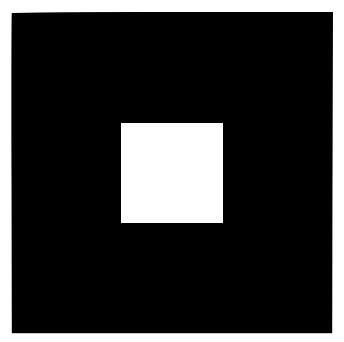
\includegraphics[width=0.3cm]{img/UTSymbols-Bullet.png}}]}
\renewcommand*{\thefootnote}{\fnsymbol{footnote}}
\newcommand{\sign}[1]{\ensuremath{\operatorname{sign(\mathit{#1})}}}

\setsansfont[Path = fonts/, UprightFont=UTSans-Medium.otf, BoldFont=UTSans-Bold.otf]{}

\title{\bf Inteligența artificială. Învățarea automată}
\author[hello@msirbu.eu]{Sîrbu Matei-Dan}
\institute[]{Universitatea Transilvania din Brașov \\ Facultatea de Matematică și Informatică}
\date{10 decembrie 2020}

\definecolor{albastruMI}{rgb}{0, 0.23, 0.49}
\setbeamercolor*{palette primary}{bg=albastruMI, fg = white}
\setbeamercolor*{palette secondary}{bg=albastruMI, fg = white}
\setbeamercolor*{palette ternary}{bg=albastruMI, fg = white}
\setbeamercolor*{palette quaternary}{bg=albastruMI, fg = white}
\setbeamercolor*{author in head/foot}{parent=palette primary}
\usefonttheme[onlymath]{serif}
\setstretch{1.5}

\begin{document}
\newcount\anim
\frame{\titlepage}

\begin{frame}
    \transfade<1>
    \frametitle{Paradigme ale învățării automate}
    \begin{itemize}
        \animate<7-15>
        \animatevalue<7-15>{\anim}{100}{0}
        \utb<1,7,8,9,10,11,12,13,14,15> {\color{black!\the\anim!blue} Învățare supervizată (supervised learning)}
        \utb<2> Învățare nesupervizată (unsupervised learning)
        \utb<3> Învățare semi-supervizată (semi-supervised learning)
        \utb<4> Învățare ranforsată (reinforcement learning)
    \end{itemize}
    \begin{itemize}
        \utb<5,6> Paradigme non-standard:
        \utb<5> Învățarea activă (active learning)
        \utb<6> Învățare prin transfer (transfer learning)
    \end{itemize}
\end{frame}

\begin{frame}
    \transdissolve<1>
    \frametitle{Învățare supervizată}
    \begin{itemize}
        \utb Avem la dispoziție exemple de obiecte etichetate
        \utb Exemplu 1: recunoașterea obiectelor din imagini cu eticheta obiectelor conținute
        \begin{center}
            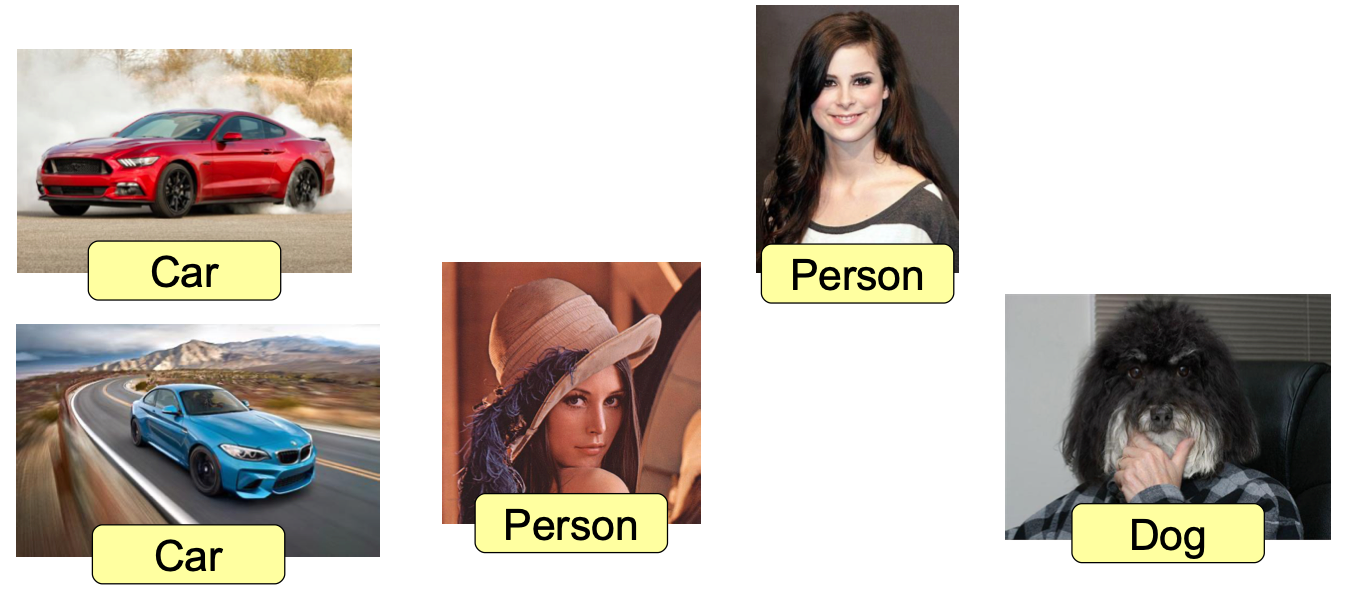
\includegraphics[width=0.9\textwidth]{img/1}
        \end{center}
    \end{itemize}
\end{frame}

\begin{frame}
    \transfade<1>
    \frametitle{Învățare supervizată}
    \begin{itemize}
        \utb Exemplu 2: recunoașterea caracterelor scrise de mână (setul de date MNIST)
        \begin{center}
            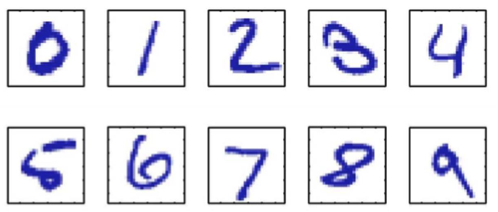
\includegraphics[width=0.35\textwidth]{img/2}
        \end{center}
        \utb Imagini de 28 $\times$ 28 de pixeli
        \utb Reprezentăm imagine ca un vector $x$ cu 784 de componente
        \utb Antrenăm un clasificator $f(x)$ astfel încât:
        \utb $f : x \rightarrow \{0, 1, 2, 3, 4, 5, 6, 7, 8, 9\}$
    \end{itemize}
\end{frame}

\begin{frame}
    \transfade<1>
    \frametitle{Învățare supervizată}
    \begin{itemize}
        \utb Exemplu 2: recunoașterea caracterelor scrise de mână (setul de date MNIST)
        \begin{center}
            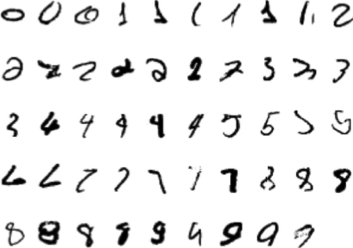
\includegraphics[width=0.28\textwidth]{img/3}
        \end{center}
        \utb Pornind de la un set de antrenare, de ex. 6000 de imagini per clasă
        \utb Rata de eroare poate ajunge la 0.23\% (cu rețele neuronale convoluționale)
        \utb Printre primele sisteme (bazate pe învățare) comerciale utilizate pe scară largă pentru procesare de coduri poștale și cecuri bancare
    \end{itemize}
\end{frame}

\begin{frame}
    \transfade<1>
    \frametitle{Învățare supervizată}
    \begin{itemize}
        \utb Exemplu 3: detectare facială
        \begin{center}
            
\includegraphics[width=0.55\textwidth]{img/4}
        \end{center}
        \utb O abordare constă în plimbarea unei ferestre peste imagine
        \utb Scopul este să clasificăm fereastra într-una din cele două clase posibile: față sau non-față (transformarea problemei într-una de clasificare)
    \end{itemize}
\end{frame}

\begin{frame}
    \transfade<1>
    \frametitle{Învățare supervizată}
    \begin{itemize}
        \utb Exemplu 3: detectare facială
        \begin{center}
            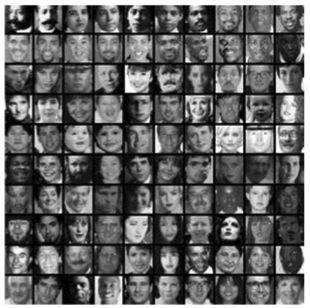
\includegraphics[width=0.3\textwidth]{img/5}
        \end{center}
        \utb Pornim de la un set cu imagini cu fețe cu diverse variații de vârstă, gen, condiții de iluminare, dar nu translație.
        \utb Și un set mult mai mare cu imagini care nu conțin fețe
    \end{itemize}
\end{frame}

\begin{frame}
    \transfade<1>
    \frametitle{Învățare supervizată}
    \begin{itemize}
        \utb Exemplu 4: detectare de spam
        \begin{center}
            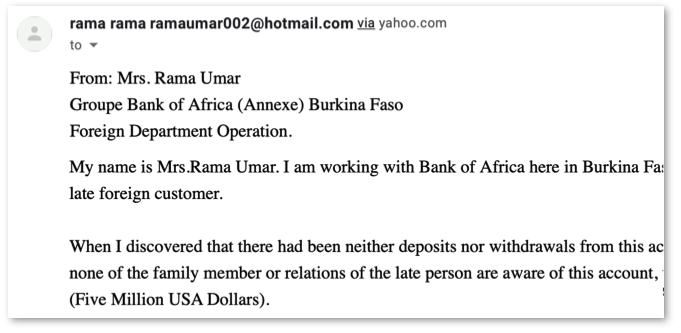
\includegraphics[width=0.6\textwidth]{img/6}
        \end{center}
        \utb Problema este de a clasifica un e-mail în spam și non-spam
        \utb Apariția cuvântului “Dollars” este un indicator de spam
        \utb Un exemplu de reprezentare este un vector cu frecvența cuvintelor
    \end{itemize}
\end{frame}

\begin{frame}
    \transfade<1>
    \frametitle{Numărăm cuvintele}
    \begin{minipage}[t!]{0.6\textwidth}
        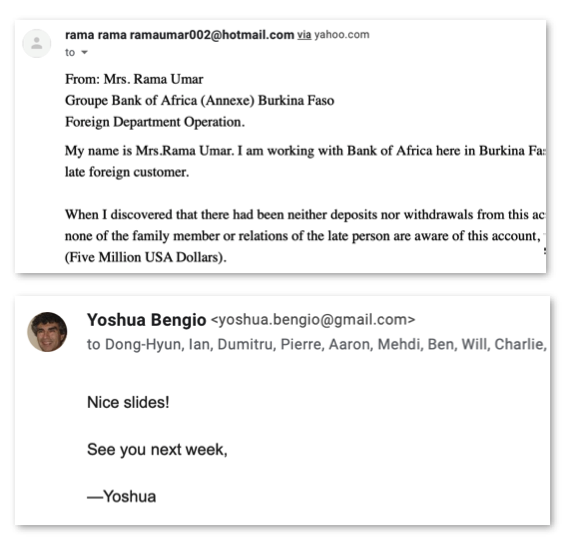
\includegraphics[width=\textwidth]{img/7}
    \end{minipage}
    \begin{minipage}[t!]{0.39\textwidth}
        \begin{center}
            \Large Obținem X \\
            \scriptsize
            $\begin{pmatrix}
                    \textrm{free}    & 100             \\
                    \textrm{money}   & 2               \\
                    \textrm{\vdots}  & \textrm{\vdots} \\
                    \textrm{account} & 2               \\
                    \textrm{\vdots}  & \textrm{\vdots}
                \end{pmatrix}$ \\
            $\begin{pmatrix}
                    \textrm{free}    & 1               \\
                    \textrm{money}   & 1               \\
                    \textrm{\vdots}  & \textrm{\vdots} \\
                    \textrm{account} & 2               \\
                    \textrm{\vdots}  & \textrm{\vdots}
                \end{pmatrix}$
        \end{center}
    \end{minipage}
\end{frame}

\begin{frame}
    \transfade<1>
    \frametitle{Algoritm de detectare a spam-ului}
    \begin{center}
        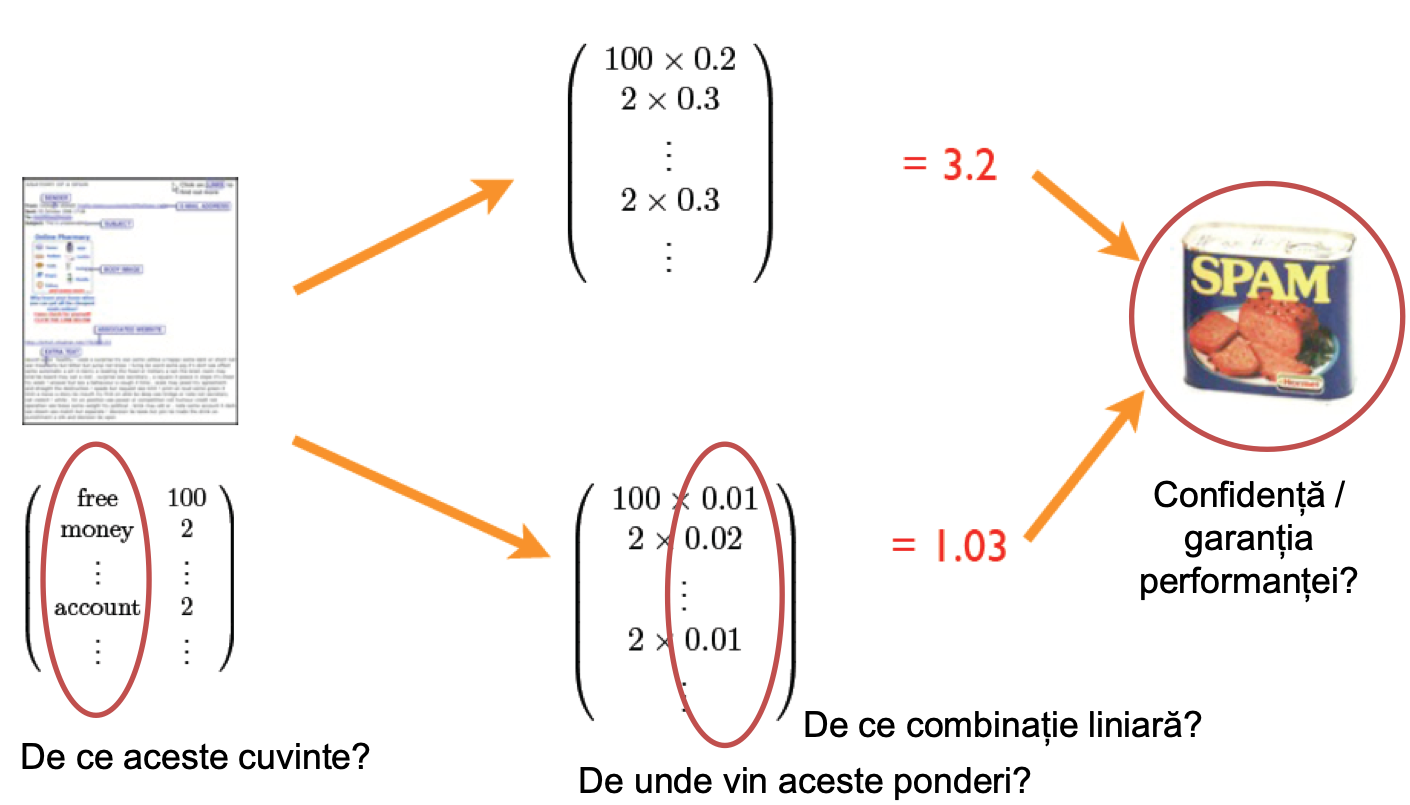
\includegraphics[width=1\textwidth]{img/8}
    \end{center}
\end{frame}

\begin{frame}
    \transfade<1>
    \frametitle{Învățare supervizată}
    \begin{itemize}
        \utb Exemplu 5: prezicerea prețului acțiunilor la bursă
        \begin{center}
            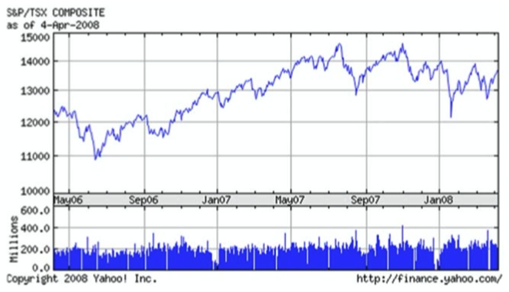
\includegraphics[width=0.45\textwidth]{img/9}
        \end{center}
        \utb Scopul este de a prezice prețul la o dată din viitor, de exemplu peste câteva zile
        \utb Acesta este un task de regresie, deorece output-ul este unul continuu
    \end{itemize}
\end{frame}

\begin{frame}
    \transfade<1>
    \frametitle{Învățare supervizată}
    \begin{itemize}
        \utb Exemplu 6: prezicerea dificultății unei imagini
        \begin{center}
            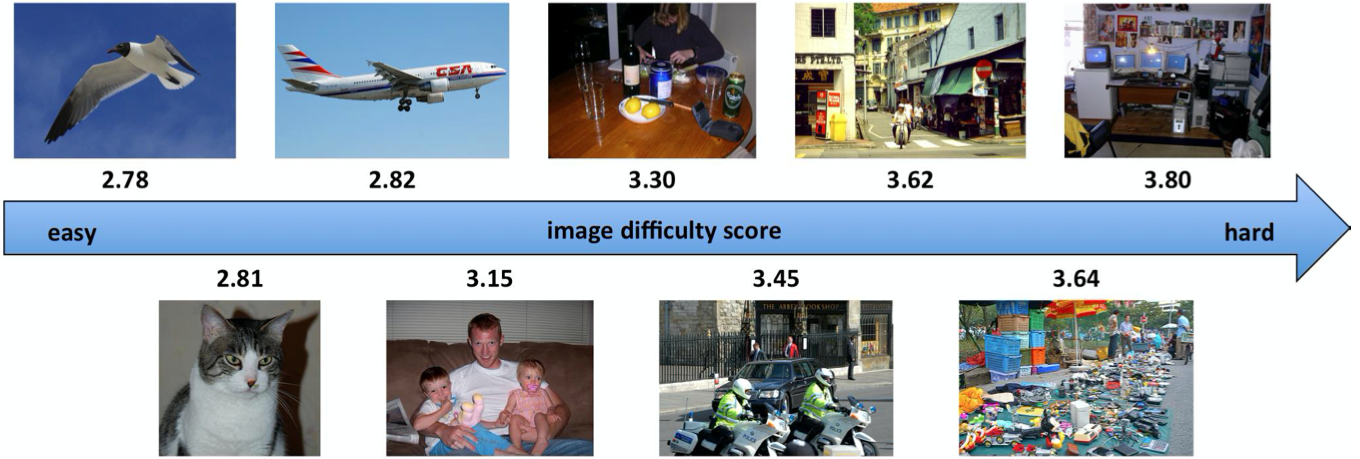
\includegraphics[width=0.9\textwidth]{img/10}
        \end{center}
        \utb Scopul este de a prezice cât de dificil ar fi pentru un om să recunoască obiectele din imagine
        \utb Acesta este un task de regresie, deorece output-ul este unul continuu
    \end{itemize}
\end{frame}

\begin{frame}
    \transfade<1>
    \frametitle{Formele canonice ale problemelor de învățare supervizată}
    \begin{itemize}
        \utb Clasificare
        \begin{center}
            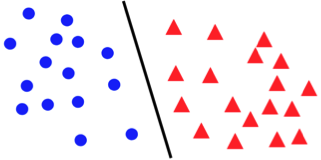
\includegraphics[width=0.35\textwidth]{img/11}
        \end{center}
        \utb Regresie
        \begin{center}
            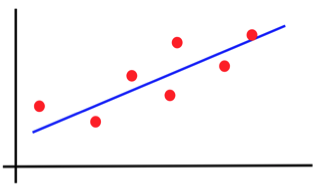
\includegraphics[width=0.35\textwidth]{img/12}
        \end{center}
    \end{itemize}
\end{frame}

\begin{frame}
    \transfade<1>
    \frametitle{Estimarea vârstei unei persoane din imagini}
    \begin{minipage}[t!]{0.7\textwidth}
        \begin{itemize}
            \utb Clasificare
            \begin{center}
                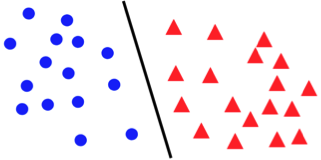
\includegraphics[width=0.5\textwidth]{img/11}
            \end{center}
            \utb Regresie
            \begin{center}
                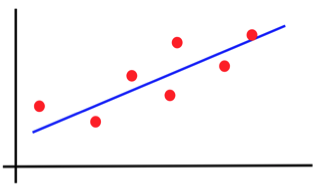
\includegraphics[width=0.5\textwidth]{img/12}
            \end{center}
        \end{itemize}
    \end{minipage}
    \begin{minipage}[t!]{0.29\textwidth}
        \begin{figure}
            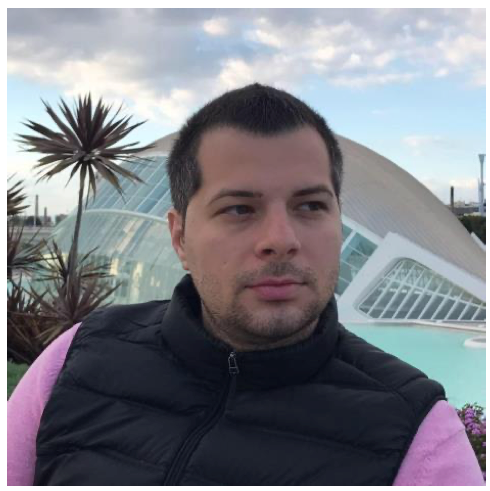
\includegraphics[width=1\textwidth]{img/13}
            \caption*{Ce vârstă?}
        \end{figure}
    \end{minipage}
\end{frame}

\begin{frame}
    \transfade<1>
    \frametitle{Paradigma de învățare supervizată}
    \begin{center}
        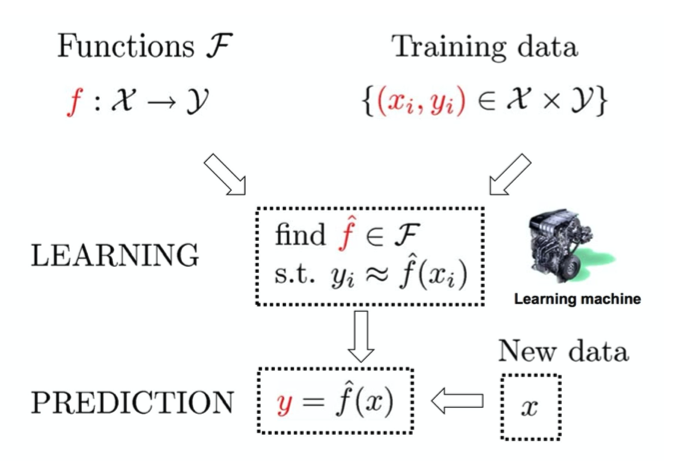
\includegraphics[width=0.8\textwidth]{img/14}
    \end{center}
\end{frame}

\begin{frame}
    \transdissolve<1>
    \frametitle{Învățare nesupervizată}
    \begin{itemize}
        \utb Avem la dispoziție exemple de obiecte fără etichete
        \utb Exemplu 1: gruparea imaginilor după similaritate
        \begin{center}
            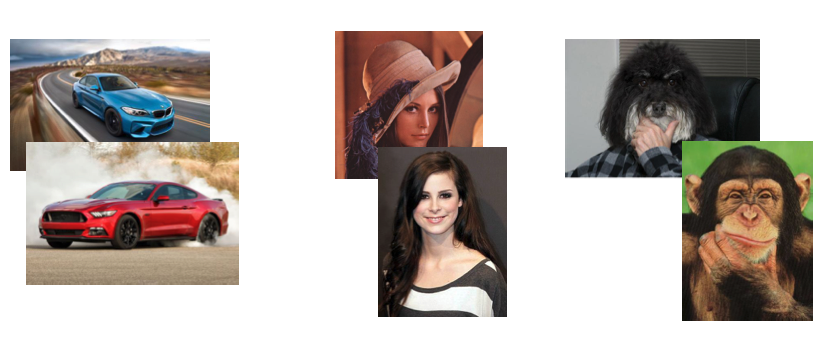
\includegraphics[width=0.9\textwidth]{img/15}
        \end{center}
    \end{itemize}
\end{frame}

\begin{frame}
    \transfade<1>
    \frametitle{Învățare nesupervizată}
    \begin{itemize}
        \utb Exemplu 2: gruparea mamiferelor pe familii, specii, etc.
        \begin{center}
            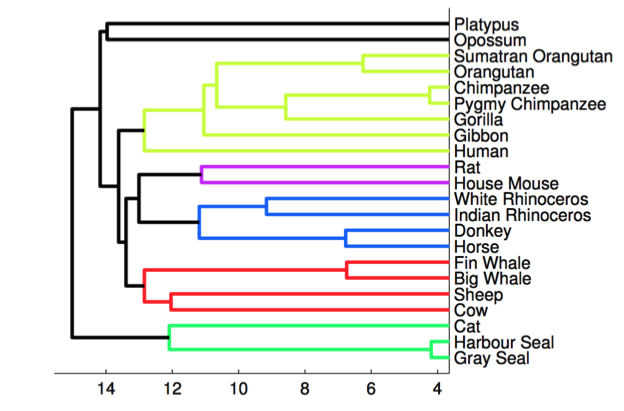
\includegraphics[width=0.65\textwidth]{img/16}
        \end{center}
        \utb Generarea arborelui filogenetic pe baza secvențelor ADN
    \end{itemize}
\end{frame}

\end{document}